
\begin{frame}
  \frametitle{Training Set Database}
  \begin{minipage}{0.43\textwidth}
    \begin{table}
      \centering
      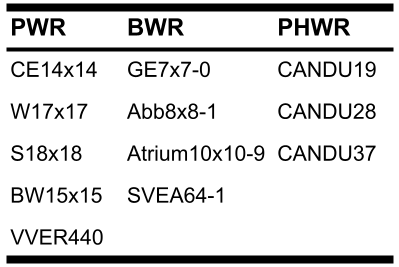
\includegraphics[width=\textwidth]{./figures/trainset4_Orxtrs.png}
      \caption{ORIGEN reactors for spent nuclear fuel simulations}
    \end{table}
  \end{minipage}%
  \hfill
  \begin{minipage}{0.53\textwidth}
    \begin{table}
      \centering
      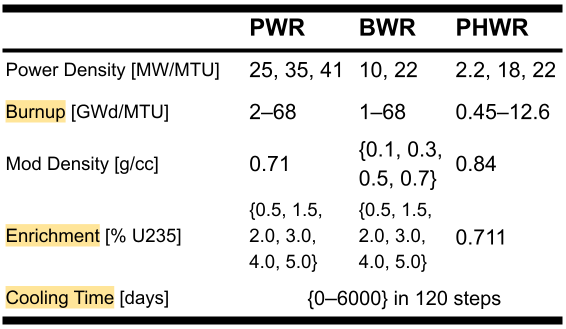
\includegraphics[width=\textwidth]{./figures/trainset4_inputs.png}
      \caption{Target reactor parameter inputs for spent fuel simulations}
    \end{table}
  \end{minipage}
\end{frame}

\begin{frame}
  \frametitle{Dimensionality Reduction: Filtering Nuclides}
    \begin{table}
      \centering
      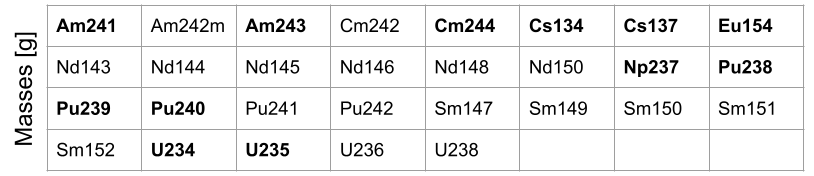
\includegraphics[width=\linewidth]{./figures/nuclist_featureset_masses.png}
      \caption{The masses of these nuclides were saved from the ORIGEN simulations}
    \end{table}
    \begin{table}
      \centering
      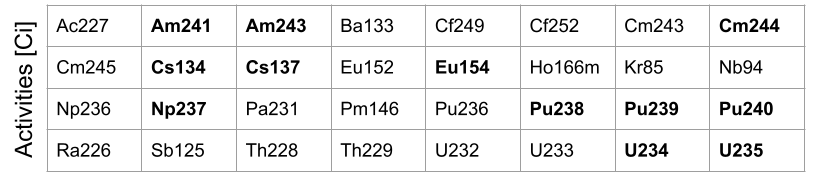
\includegraphics[width=\linewidth]{./figures/nuclist_featureset_activities.png}
      \caption{The activities of these nuclides were saved from the ORIGEN simulations}
    \end{table}
\end{frame}

%\begin{frame}
%  \frametitle{Visualizing the Database}
%  \bigskip
%  \centering Linear Discriminant Analysis \\ \bigskip
%  \begin{minipage}{0.5\textwidth}
%    \begin{table}
%      15 isotopes
%      \centering
%      \includegraphics[width=\linewidth]{./figures/lda-trainset_15nuc.png}
%    \end{table}
%  \end{minipage}%
%  \begin{minipage}{0.5\textwidth}
%    \begin{table}
%      10 ratios
%      \centering
%      \includegraphics[width=\linewidth]{./figures/lda-trainset_10ratios.png}
%    \end{table}
%  \end{minipage}
%\end{frame}

\begin{frame}
  \frametitle{Information Reduction}
  \textbf{\large Random \& Uniform Error} \\
  \bigskip
  \textit{Machine Learning Algorithms} \\ \smallskip
  Introduced $0.0 < E_{max} < 0.2$ random error\\
  Each nuclide measurement receives $[1-E_{max},1+E_{max}]$\\
  \bigskip
  \textit{Maximum Likelihood Calculations} \\ \smallskip
  Introduced uniform simulation uncertainty\\
  Each nuclide measurement is given a standard deviation of $5\%$, $10\%$, $15\%$, $20\%$ \\
\end{frame}

\begin{frame}
  \frametitle{Information Reduction}
  \textbf{\large Detector Response \& Systematic Error} \\
  \medskip
  \begin{enumerate}
    \item Reduced radionuclide observation using nuclide activities to obtain gamma spectra
    \item Choose energy windows / window size
    \item Counting error ($\sqrt{n}$) injected using method on previous slide
    \item Decrease detector energy resolution
  \end{enumerate}
  \begin{figure}[h!]
    \centering
    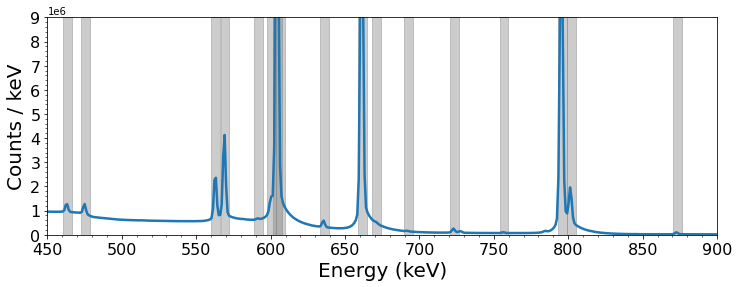
\includegraphics[height=0.4\textheight]{./figures/energy_window_example.png}
    \caption{Illustration of step 2 of the process outlined above}
  \end{figure}
\end{frame}
